\documentclass[10pt]{article}
\usepackage[letterpaper, margin=0.6in]{geometry}
\usepackage{graphicx}
\usepackage{booktabs}
\usepackage[font=small, labelfont=bf, skip=4pt]{caption}
\usepackage{microtype}
\usepackage[hidelinks]{hyperref}
\hypersetup{pdftitle={Lab 1: Interactive Image Mosaic Generator}, pdfauthor={Pinar Aksoy}}
\usepackage{titlesec}
\titlespacing*{\section}{0pt}{6pt}{2pt}
\titlespacing*{\paragraph}{0pt}{2pt}{0.6em}
\setlength{\textfloatsep}{6pt}
\setlength{\intextsep}{6pt}
\graphicspath{{../results/}}

\begin{document}

\begin{center}
  {\Large\bfseries Lab 1: Interactive Image Mosaic Generator}\\[4pt]
  Pinar Aksoy \quad CS5130, Fall 2026 \quad Code: \url{https://github.com/0xpinara/mosaic-hf}\\[2pt]
  Live demo: \url{https://huggingface.co/spaces/piax0x/mosaic-hf}
\end{center}
\suppressfloats[t]

\section{Method}

\paragraph{Preprocessing.}
All the image processing is in \texttt{mosaic.py}. The grid size $N$ is the number of tiles along the longer side of the image, and each cell is $\lfloor 1024/N \rfloor$ pixels wide (32~px for $N=32$). The image is resized so its long side is exactly $N$ cells, and the short side is center-cropped to a whole number of cells, so less than one cell is cut off. This gives a fixed working resolution for each $N$ (1024~px on the long side when $N$ divides 1024, 960~px for $N=96$).

\paragraph{Grid analysis and classification.}
To get the mean color of every cell without loops, I reshape the $H \times W \times 3$ image into a $(\mathit{rows}, \mathit{cell}, \mathit{cols}, \mathit{cell}, 3)$ array. The pixels of each cell are then on axes 1 and 3, and one \texttt{mean(axis=(1,3))} returns all the cell colors at once. The $k$ color categories come from k-means color quantization (\texttt{cv2.kmeans}, k-means++ initialization, fixed seed) on these cell colors rather than on every pixel. I cluster and match in CIELAB, where distances are closer to how different two colors look than in RGB. Subtracting the $(1, k, 3)$ category colors from a $(\mathit{cells}, 1, 3)$ array gives every distance in one step, and \texttt{argmin} gives each cell a category label, so the category boundaries act as color thresholds. Above 4096 cells, k-means runs on a random sample of 4096 cells (8~ms instead of 32~ms at $128 \times 128$). The segmented image shows each cell in its category color (Fig.~\ref{fig:tiles}b).

\paragraph{Tiles.}
The tile patterns are drawn once at $128 \times 128$~px and shrunk to the cell size, and all $k$ tiles are made at once by broadcasting the category colors against the pattern. The mosaic is \texttt{tiles[labels]}, a $(\mathit{rows}, \mathit{cols}, \mathit{cell}, \mathit{cell}, 3)$ array that is transposed and reshaped back into an image, so nothing loops over the cells. There are five tile sets (Fig.~\ref{fig:tiles}). \emph{LEGO bricks} multiply the color by the shading of a $1 \times 1$ brick seen from above (beveled edges and a shaded stud). \emph{Flat colors} are plain squares and serve as the baseline. \emph{Dots} are round beads on a dark background, like an LED board. \emph{ASCII} uses intensity thresholding: the brightness range is cut into 11 levels, one for each character (sorted by how much ink it uses), so brighter cells get denser characters, drawn in the category color on a near-black background. \emph{Photo tiles} skip k-means and make a real photomosaic: the seven test photos are cut into 592 patches of $64 \times 64$~px, each cell gets the patch with the closest mean color, and the patch is shifted 40\% toward the cell's color. When the input is one of the test photos (found by comparing thumbnails, so renamed copies count too), its own patches are left out; before I added this, the astronaut at an $8 \times 8$ grid came back almost unchanged (SSIM 0.999).

\begin{figure}[tb]
  \centering
  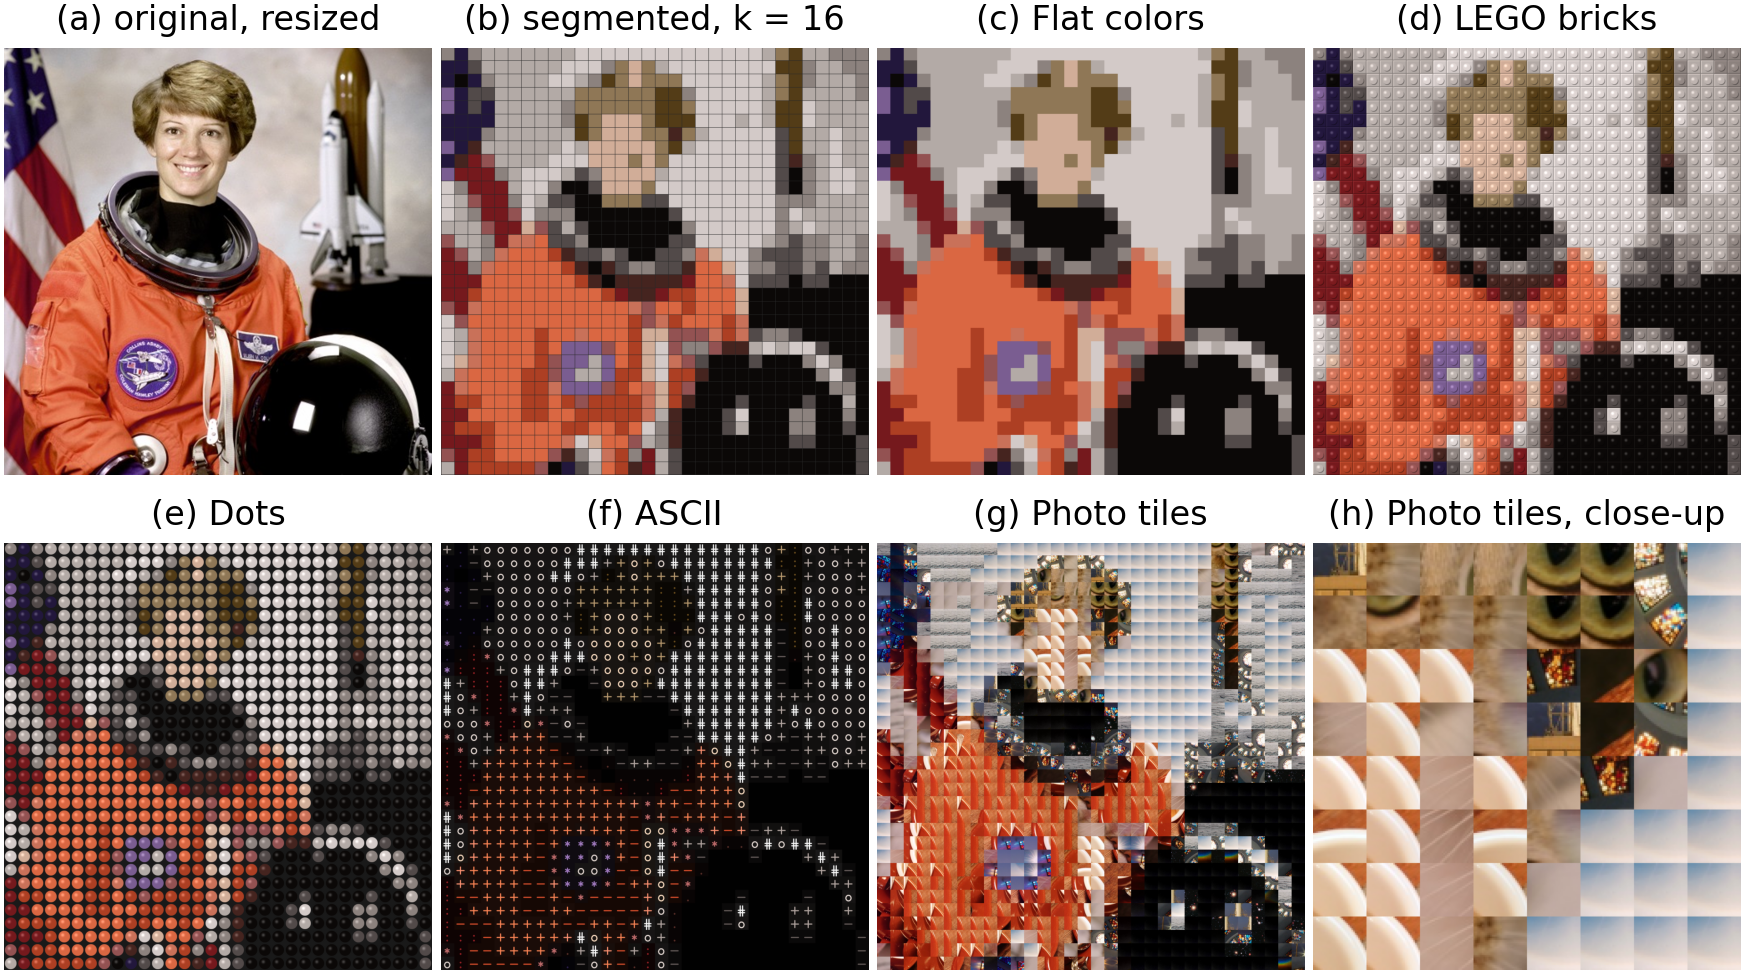
\includegraphics[width=0.66\textwidth]{figure_tile_sets.png}
  \caption{Astronaut image with a $32 \times 32$ grid and $k = 16$: (a) resized original, (b) segmented image, (c)--(g) the five tile sets, (h) close-up of (g); its patches come from the other six photos.}
  \label{fig:tiles}
\end{figure}

\paragraph{Interface.}
The Gradio app (\texttt{app.py}) has an image upload, a slider for the grid size (8 to 128), a dropdown for the tile set and a slider for $k$. It shows the resized original and the segmented image next to each other, the mosaic below them, and then MSE, SSIM and the processing time. It updates whenever the user changes an input (sliders when they are released). Eight clickable examples cover all seven test images and all five tile sets (Fig.~\ref{fig:examples} uses the same settings), and the app runs on Hugging Face Spaces with pinned library versions.

\begin{figure}[tb]
  \centering
  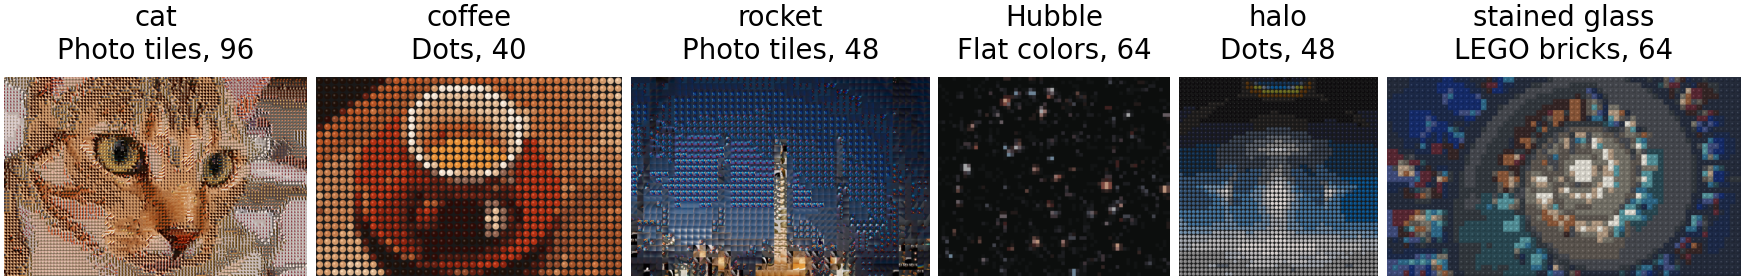
\includegraphics[width=0.9\textwidth]{figure_examples.png}
  \caption{The other six test images, with the tile set and grid size above each one ($k = 16$).}
  \label{fig:examples}
\end{figure}

\section{Similarity metrics}
I compare the mosaic with the resized original (same size) using MSE on the 0 to 255 RGB values (lower is better) and SSIM from scikit-image ($7 \times 7$ window, mean over the three channels). SSIM compares local brightness, contrast and structure instead of single pixels, and is 1 for identical images. Table~\ref{tab:sim} averages both over the seven test images, center-cropped to squares so every grid is exactly $N \times N$.

\begin{table}[!htb]
  \centering
  \caption{MSE and SSIM between original and mosaic by grid size (mean of 7 images, $k = 16$).}
  \label{tab:sim}
  \small
  \begin{tabular}{l rrrr rrrr}
    \toprule
    & \multicolumn{4}{c}{MSE (lower is better)} & \multicolumn{4}{c}{SSIM (higher is better)} \\
    \cmidrule(lr){2-5} \cmidrule(lr){6-9}
    Tile set & $16^2$ & $32^2$ & $64^2$ & $128^2$ & $16^2$ & $32^2$ & $64^2$ & $128^2$ \\
    \midrule
    Flat colors & 990  & 661  & 443  & 287  & 0.618 & 0.625 & 0.637 & 0.678 \\
    LEGO bricks & 1265 & 930  & 692  & 444  & 0.405 & 0.319 & 0.256 & 0.304 \\
    Dots        & 3561 & 3300 & 3098 & 2722 & 0.406 & 0.303 & 0.189 & 0.155 \\
    ASCII       & 7871 & 7626 & 7326 & 6996 & 0.198 & 0.183 & 0.159 & 0.136 \\
    Photo tiles & 3150 & 2578 & 2201 & 1763 & 0.284 & 0.236 & 0.185 & 0.162 \\
    \bottomrule
  \end{tabular}
\end{table}

MSE drops for every tile set as the grid gets finer, because smaller cells follow the image more closely (Flat colors: 990 at $16 \times 16$, 287 at $128 \times 128$), and Flat colors always score best since any texture inside a tile counts as error. SSIM behaves differently: for the four textured sets it drops as the grid gets finer (Dots: 0.406 to 0.155) even though MSE improves, because the texture inside the tiles becomes the main local structure and does not match the photo. LEGO recovers a little at $128 \times 128$, where shrinking the brick to 8~px softens its shading. Photo tiles are third in MSE but near the bottom in SSIM: their colors match each cell only on average, and their edges rarely match those in the image. With an image's own patches allowed they scored much higher (SSIM 0.417 instead of 0.236 at $32 \times 32$), but only because the mosaic partly reused the image. ASCII is last because most of each tile is near-black.

The images differ a lot too: at $32 \times 32$ with Flat colors, the rocket (MSE 221) and the halo (253) are easy because they are mostly smooth sky, while the astronaut (1360) and the stained glass (1157) are the hardest, since their high-contrast details (flag stripes, badges, pieces of glass) are smaller than a cell. So the metrics measure closeness to the original rather than how good a mosaic looks; to me LEGO and Photo tiles look better than their scores suggest.

\section{Performance}
I timed the grid operations (cell colors, classification and tile placement) with \texttt{benchmark.py} on the seven images, cropped to squares and resized to $1024 \times 1024$~px. A loop version does the same steps with two nested \texttt{for} loops over the cells and gives exactly the same mosaic (checked with \texttt{np.array\_equal} for every image and grid). Values are medians of repeated runs, averaged over the images, on my Apple M2 Mac (Python 3.12, NumPy 2.4.4, OpenCV 4.13).

\begin{table}[!htb]
  \centering
  \caption{Processing time per grid size in ms (average of the 7 images, $1024 \times 1024$~px, LEGO bricks, $k = 16$).}
  \label{tab:time}
  \small
  \begin{tabular}{l r r r r r r r}
    \toprule
    Grid & Cells & Cell size & Vectorized & Nested loops & Speedup & Full pipeline & Metrics \\
    \midrule
    $8 \times 8$     & 64     & 128 px & 10.8 & 11.4  & 1.1$\times$ & 23.3 & 249.3 \\
    $16 \times 16$   & 256    & 64 px  & 10.9 & 12.0  & 1.1$\times$ & 20.2 & 228.7 \\
    $32 \times 32$   & 1024   & 32 px  & 10.8 & 17.4  & 1.6$\times$ & 19.6 & 203.0 \\
    $64 \times 64$   & 4096   & 16 px  & 12.7 & 41.6  & 3.3$\times$ & 29.3 & 212.8 \\
    $128 \times 128$ & 16384  & 8 px   & 19.6 & 140.7 & 7.2$\times$ & 37.7 & 213.3 \\
    \bottomrule
  \end{tabular}
\end{table}

The vectorized time hardly depends on the grid size: the number of cells grows 256 times from $8 \times 8$ to $128 \times 128$, but the time only goes from 10.8 to 19.6~ms, since most of the work is per pixel and the pixel count is fixed. The loop version needs about 11~ms of pixel work plus roughly 8~\textmu s of Python overhead per cell (a slice, a mean, a color conversion and an argmin). With few cells that overhead does not matter (1.1$\times$ at $8 \times 8$), but for big grids it takes over: from $64 \times 64$ to $128 \times 128$ the cells grow 4$\times$ and the loop time 3.4$\times$, and at $128 \times 128$ the vectorized code is 7.2$\times$ faster. The full pipeline (resizing, k-means, tiles, segmented image) takes 20 to 38~ms, so the MSE and SSIM step (about 0.2~s) is the slowest.

\section{Conclusion}
The generator works on images of any size and aspect ratio and is fast enough to feel interactive. The metrics show a trade-off between accuracy and style: the more interesting tile sets lose points for the texture that makes them look like mosaics. Next I would add a bigger photo library, since the same patches repeat and need a strong color shift.

\end{document}
